\chapter{\IfLanguageName{dutch}{Stand van zaken}{State of the art}}
\label{ch:stand-van-zaken}

% Tip: Begin elk hoofdstuk met een paragraaf inleiding die beschrijft hoe
% dit hoofdstuk past binnen het geheel van de bachelorproef. Geef in het
% bijzonder aan wat de link is met het vorige en volgende hoofdstuk.

% Pas na deze inleidende paragraaf komt de eerste sectiehoofding.

Dit onderzoek richt zich op automatische \textit{machine learning} platformen. Maar alvorens van start te gaan met de onderliggende technieken is het belangrijk om een goed zicht te hebben op de basis waarop het gebouwd is. Zo worden eerst een aantal belangrijke begrippen en technieken besproken, deze sectie kan overgeslagen worden als deze intro triviaal is voor de lezer. De automatisatie hiervan wordt onderzocht, welke technieken worden met elkaar gecombineerd en hoe bekom je uiteindelijk resultaten. Het is nodig om de theoretische benadering goed te begrijpen om uiteindelijk te kunnen beslissen als het resultaat van het experiment voldoet aan de normen van een goed werkend model. Tot slot worden de beschikbare cloud platformen besproken en vergeleken met een open source libraries als alternatief.

\section{Inleiding machine learning}
\label{sec:inl-machine-learning}

Deze sectie dient om mensen zonder kennis van machine learning bekend te maken met enkele begrippen en technieken binnen het werkveld. Mensen met enige basiskennis kunnen direct doorgaan naar de volgende sectie.

Het is belangrijk dat volgende begrippen gekend zijn:
\begin{itemize}
    \item \textbf{Data Cleaning / Cleansing}: Het detecteren, corrigeren of verwijderen van onnauwkeurige datarecords. Het resultaat is een consistente dataset die bruikbaar is om een model te trainen
    \item \textbf{Feature Selection}: Het selecteren van relevante kolommen uit de dataset. Het zijn de belangrijkste eigenschappen die de voorspelling bepalen
    \item \textbf{Software agent}: Een computerprogramma die in staat is om te leren uit eerdere ervaringen
\end{itemize}

\subsection{Soorten machine learning}
\label{subsec:soorten-machine-learning}

\begin{figure}
    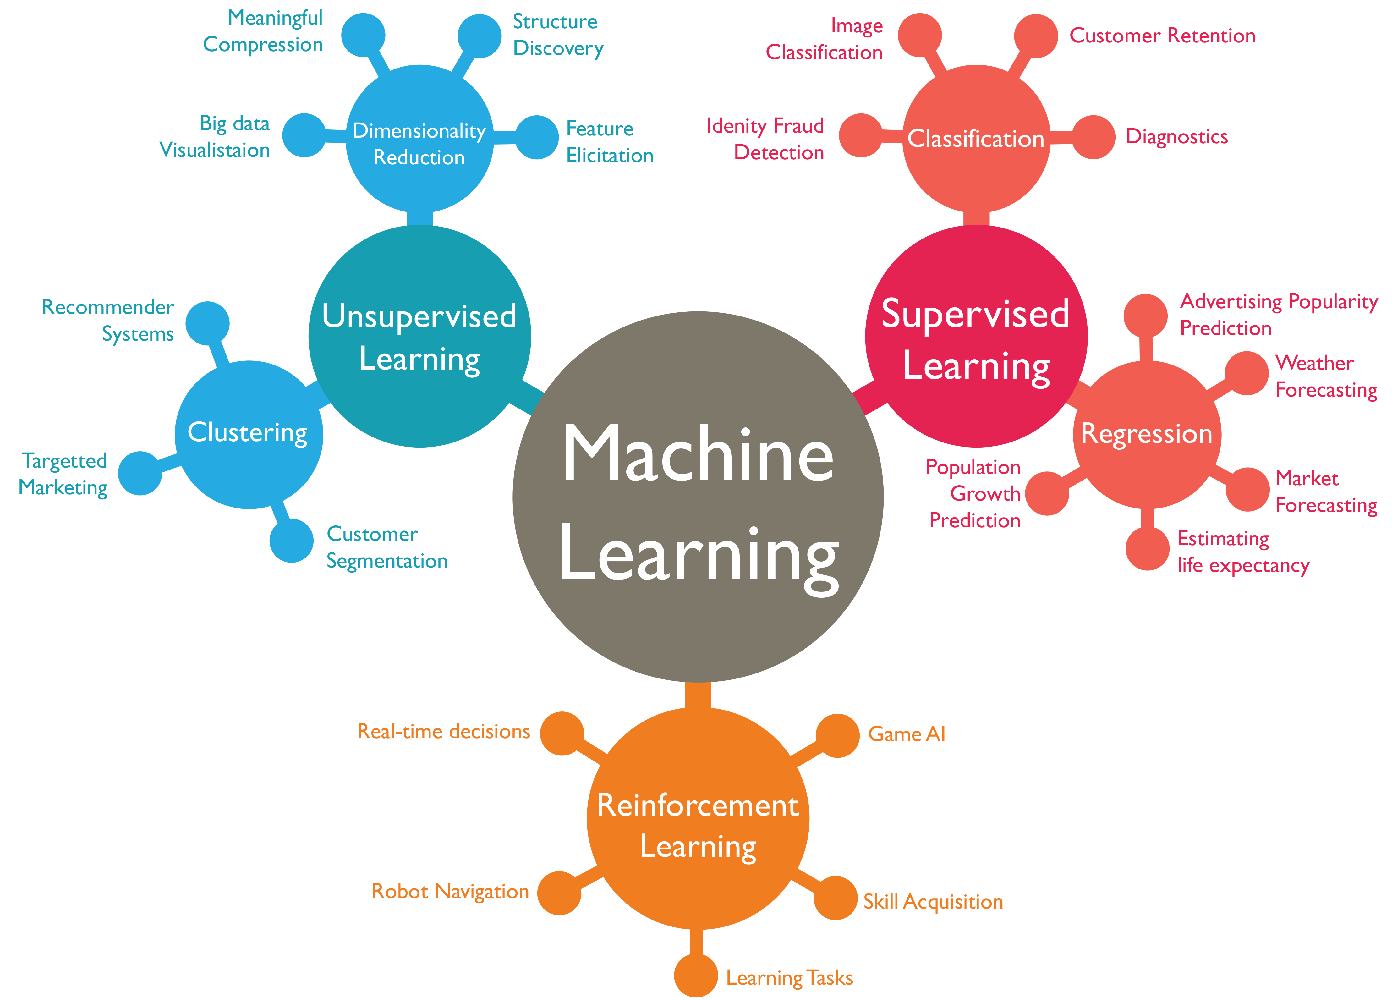
\includegraphics[width=\linewidth]{img/ml-soorten.png}
    \caption{Soorten machine learning met enklele toepassingen \autocite{Arroyo2017}}
    \label{fig:ml-soorten}
\end{figure}

\textcite{Lievens2019} schreef over 3 grote types binnen het domein van machine learning. Deze worden kort verklaard aan de hand van een praktisch voorbeeld. Figuur \ref{fig:ml-soorten} is een algemeen overzicht van wat hieronder beschreven is.


\subsubsection{Gesuperviseerd leren}
\label{subsubsec:gesuperviseerd-leren}

Bij gesuperviseerd leren probeert de software agent een functie te leren die een voorspelling maakt voor een gegeven input. De functie die deze voorspellingen maakt evolueert door het gebruik van een trainingsdataset met input-output waarden \autocite{Norvig1994}.

Classificatie is een typisch probleem dat opgelost wordt met gesuperviseerd leren, het wordt later in dit onderzoek op een andere manier opgelost. Het doel van classificatie is om aan de hand van enkele kenmerken een voorgedefinieerde klasse te voorspellen. Er wordt gesproken van een binair classificatieprobleem als er slechts 2 klassen zijn. Spamdetectie is hier een voorbeeld van. Door de belangrijke woorden uit een bericht te halen wordt er een attribuutvector opgebouwd. Door een model te trainen met duizenden berichten en als ze al dan niet spam zijn, kan het een voorspelling maken voor de gegeven vector \autocite{Lievens2019}.

\subsubsection{Ongesuperviseerd leren}
\label{subsubsec:ongesuperviseerd-leren}

Met ongesuperviseerd leren is het mogelijk om in een ongelabelde dataset patronen te vinden die eerder onbekend waren. Bij elke voospelling wordt voor elke categorie meegegeven hoe zeker het model is over zijn voorspelling \autocite{Hinton1999}.

Een ongelabelde dataset met gegevens over klanten waarvoor je te weten wilt komen als er onderliggende groepen ontdekt kunnen worden. Dit wordt ook clustering genoemd, een mogelijke oplossing is \autocite{Lievens2019}:

\begin{itemize}
    \item Klanten die waarschijnlijk hun contract verlengen.
    \item Ontevreden klanten die bijna zeker hun contract opzeggen.
    \item Klanten die voor een bepaalde aanbieding misschien hun contract verlengen.
\end{itemize}

Deze resultaten worden bekomen door berekeningen uit te voeren op de attribuutvector zonder een outputlabel. Deze techniek is, in het kader van dit onderzoek, minder relevant.

\subsubsection{Reinforcement Learning}
\label{subsubsec:reinforcement-learning}

Reinforcement learning focust zich op de acties die een software agent onderneemt om een zo hoog mogelijke beloning te krijgen. Er is dus geen nood aan een (gelabelde) dataset zoals bij gesuperviseerd en ongesuperviseerd leren. De agent probeert een balans te vinden tussen wat hij weet en wat er kan gebeuren \autocite{Kaelbling1996}. In essentie wil dit zeggen dat de agent probeert te leren welke acties leiden tot de hoogste totale beloning \autocite{Lievens2019}.

Deze techniek wordt verder besproken in het deel over geautomatiseerde machine learning.


Geautomatiseerde \textit{machine learning} is het automatiseren van het trainingsproces bij een artificieel neuraal netwerk. De lage toegangsdrempel zorgt ervoor dat mensen met beperkte \textit{machine learning }kennis sneller en simpeler een model kunnen trainen en gebruiken.

\subsubsection{Transfer Learning}
\label{subsubsec:transfer-learning}

\begin{figure}
    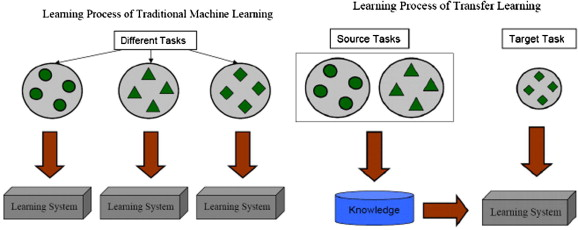
\includegraphics[width=\linewidth]{img/transfer-learning.jpg}
    \caption{Informatieoverdracht bij Transfer Learning \autocite{Pan2009}.}
    \label{fig:transfer-learning}
\end{figure}

Een andere manier om een neuraal netwerk te trainen is eerst een gegeneraliseerd model maken en die later specifiek toepassen op de situatie waarin het zich bevindt. Het idee achter transfer learning komt hierop neer, een gegeneraliseerd model kan vormen, kleurveranderingen en hoeken herkennen. Door de laatste lagen van het model af te knippen en nieuwe meer gespecialiseerde lagen toevoegt, zeg je in principe welke soort van de opgesomde eigenschappen het moet herkennen \autocite{Khandelwal2019}. 

In figuur \ref{fig:transfer-learning} is zichtbaar hoe een traditioneel model verschilt van een model getraind met transfer learning. Voor verschillende taken hoeft het niet volledig opnieuw getraind worden (op voorwaarde dat het binnen de generalisatie valt) en kan je de laatste lagen fine-tunen naar wens. Zo kan een model getraind worden om voertuigen te herkennen en later gespecialiseerd worden naar bijvoorbeeld auto's, vrachtwagens, fietsen of moto's.

\section{Proces model bij data analyse}
\label{sec:proces-model}

\begin{figure}
    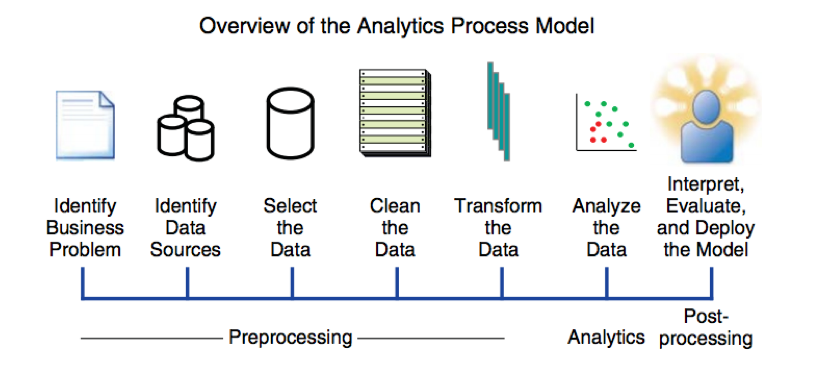
\includegraphics[width=\linewidth]{img/proces-model.png}
    \caption{Verschillende stappen in een data analyse project \autocite{Lemahieu2018}}
    \label{fig:proces-model.png}
\end{figure}

Volgens \textcite{Lemahieu2018} bestaat elk data analyse project uit 7 verschillende stappen, in de gegeven volgorde van figuur \ref{fig:proces-model.png}. Er wordt aangenomen dat 80-90\% van de totale tijd gespendeerd wordt aan \textit{preprocessing} van de data. Voordat een AutoML systeem bruikbaar is in de situatie van dit onderzoek moet het in staat zijn om de initiële stap uit te voeren. Het identificeren van het business probleem en de \textit{data sources} mogen al uitgesloten worden, de opdracht die een \textit{development} team krijgt bevat idealiter alle informatie. 

We zijn dus niet enkel op zoek naar een oplossing die analyses kan uitvoeren en interpreteren, maar ook naar iets dat data op een correcte manier kan behandelen zodat er een autonoom systeem gevormd wordt. 

\section{Neural Architecture Search}
\label{sec:nas}

\begin{figure}
    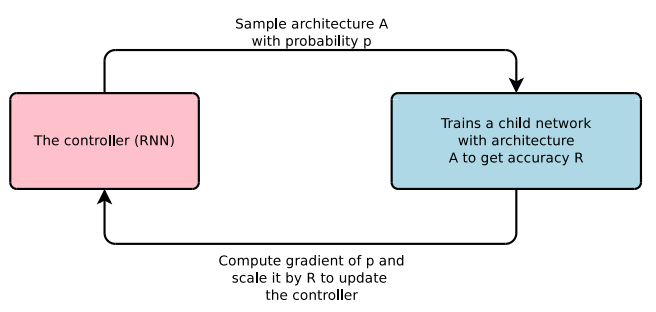
\includegraphics[width=\linewidth]{img/nas.png}
    \caption{Werking van Neural Architecture Search \autocite{ZophL2016}}
    \label{fig:nas-bp}
\end{figure}

Dergelijke geautomatiseerde machine learning systemen gebruiken een techniek die het ontwerp van een artificieel neuraal netwerk kan automatiseren, beter bekend als \textit{Neural Architecture Search} \autocite{Elsken2019}. De benaming verklapt al wat de kerntaak is, het zoeken naar de optimale netwerkarchitectuur optimaliseren. Uit \textcite{ZophL2016} wordt vastgesteld dat deze techniek een gelijkaardige of zelfs betere performantie heeft op een vaak gebruikte dataset dan modellen die door een ML-ingenieur ontworpen zijn.

\textit{Neural Architecture Search} is een kostelijk algoritme om uit te voeren op een grote dataset. De verkregen resultaten uit \textcite{ZophL2016} hebben enkele weken geduurd met 800 GPU's. Daarom wordt er in \textcite{Zoph2017} voorgesteld om een model te trainen voor een (kleinere) proxy dataset en die aan de hand van \textit{transfer learning} te extraheren naar de volledige dataset. Door op voorhand een zoekruimte te definiëren is de complexiteit van de architectuur losstaand van de diepte van het model en de grootte van de afbeeldingen. Met andere woorden wordt er dus gezocht naar de beste lagenstructuur, want die blijven onveranderd bij het transfereren van het model. Deze aanpak komt veel sneller tot zijn resultaat want enkel de gewichten moeten aangepast worden.

De technieken uit Sectie \ref{sec:hyperparameter-tuning} zijn onderliggend verwerkt en spelen een belangrijke rol binnen het domein van machine learning \autocite{ZophL2016}. \textit{Reinforcement Learning} is een populaire zoekstrategie maar andere zoek- en optimalisatiealgoritmen zoals bijvoorbeeld \textit{Bayesian optimization} zijn ook mogelijk \autocite{Elsken2019}.

\subsubsection{Gebruik van Reinforcement Learning}
\label{subsubsec:nas-reinforcement}

Neural Architecture Search gebruikt Reinforcement Learning om een model te trainen. Deze manier van werken is fundamenteel anders dan gesuperviseerd / ongesuperviseerd leren omdat het model niet beter wordt door het gebruik van datasets. Als alternatief kan het neuraal netwerk beloningssignalen herkennen waardoor het kan leren welke acties leiden tot een positief resultaat \autocite{Lievens2019}.

Op figuur \ref{fig:nas-bp} wordt gevisualiseerd hoe dit werkt. Op basis van controller structuur A (waarbij A een neuraal netwerk is) wordt een string met variabele lengte gegenereerd. Deze waarden worden gebruikt als hyperparameters om een kind-netwerk aan te maken, die getraind wordt met echte data en waarbij de accuraatheid gemeten wordt aan de hand van een validatie dataset. Het resultaat wordt gebruikt als beloningssignaal voor de controller, bij de volgende iteratie kan deze hogere kansen geven aan parameters die leiden tot accurate voorspellingen \autocite{ZophL2016}. De controller zijn zoekfunctie zal dus verbeteren over tijd.

\subsubsection{Verbeteringen met Network Morphism}
\label{subsubsec:network-morphism}

In de tweede alinea van sectie \ref{sec:nas} is al gesproken over de grote hoeveelheid resources die nodig zijn om tot de voorgestelde resultaten te komen. De afhankelijkheid van die resources zorgt ervoor dat er geen praktische manier is om het systeem te gebruiken als die capaciteiten niet beschikbaar zijn \autocite{Cai2017}. \textcite{Cai2017} zegt dat het verlies in performantie komt omdat elk kind-netwerk volledig vanaf nul getraind wordt, zonder kennis te hebben van vorige bewandelde paden. De technologie is bewezen, de moeilijkheid bevindt zich nu in het reproduceren met minder rekenkracht.

Denk maar aan hoe menselijke expertise tot stand komt. De herhalende taakt moet kennis opleveren over de gekozen gewichten, architectuur en meer \autocite{Chen2016}. Dit zonder telkens gereset te worden.

\textit{Network Morphism} tracht de bestaande kennis van een model uit te breiden door netwerkoperaties uit te voeren (lagen toevoegen, uitbreiden ...) zonder het oorspronkelijk model aan te passen \autocite{Cai2017}. Met een voorgedefinieerde transformatie functie kan bestaande kennis in een nieuw model gepompt worden zodat het dezelfde taak kan uitvoeren. Met andere parametrisatie gecombineerd met het gebruik van \textit{reinforcement learning} (zie sectie \ref{subsubsec:reinforcement-learning}) bekom je volgens \textcite{Cai2017} een \textit{meta-controller} met verbeterde performantie.

\section{Hyperparameter tuning}
\label{sec:hyperparameter-tuning}

In de vorige sectie is het gebruik van parameters aan bod gekomen. Neural Architecture Search en Hyperparameter tuning zijn dan ook sterk gerelateerd aan elkaar. De normale parameters bepalen het gedrag van een neuraal netwerk en hebben een grote invloed op het eindresultaat. Het gegeven gewicht aan een parameter stelt, zoals eerder vermeld, hoe groot de invloed is van deze laag / neuron op de voorspelling. \textcite{GoogleHT2020} verduidelijkt dat Hyperparameters eigen zijn aan de configuratie en niet aan het model. Zo moet er bepaald worden hoeveel lagen en het aantal neuronen per laag er zijn. Tijdens het trainen blijven deze constant. Volgens \textcite{Brust2019} zijn er verschillende manieren om de hyperparameters te optimaliseren. \textit{Brute force} zal elke configuratie overlopen en beslissen hoe het model vordert terwijl \textit{feature selection} gewichten aan verschillende hyperparameters geeft. Op die manier hebben vorige simulaties een impact bij de selectie van een nieuwe set hyperparameters \autocite{Claesen2015}. In \textcite{Bergstra2011} wordt nog gesproken over \textit{Random Search} die in sommige gevallen dezelfde (slechte) performantie heeft als \textit{Brute force}, en de meer gesofisticeerde methodes die verder besproken worden. 

\textcite{ZophL2016} stelt dat deze methoden in het algemeen minder goed werken dan Neural Architecture Search, dit is omdat de netwerk configuraties gevormd worden in een zoekruimte met vaste lengte. Bayesian optimization \autocite{Bergstra2013}, een variant van hyperparameter tuning, werkt wel met variabele zoekruimtes maar blijven minder flexibel dan wat er voorgesteld wordt bij Neural Architecture Search. In de praktijk bekomt men wel vaak een goed resultaat als er een initieel model bijgeleverd wordt \autocite{ZophL2016}.

\subsection{Meta-learning}
\label{subsec:meta-learning}

De principes achter de systemen die zelf leren en verbeteren komt uit \textcite{Schmid1987}. Het doel ervan is om aan de hand van randinformatie te begrijpen hoe leerproblemen flexibel worden. Die kennis kan verder ook gebruikt worden om herhalende taken te verbeteren over tijd \autocite{ZophL2016}. De typische benaming is 'leren leren'.

Randinformatie in deze situatie wordt ook metadata genoemd. Dit is niet meer dan informatie over andere data. Voorbeelden van metadata kunnen zijn: eigenschappen van het algoritme (\textit{metrics} die de performantie meten) of informatie over het probleem. In \textcite{Schmidhuber1993} wordt het principe getoond waarbij een zelf refererend neuraal netwerk zijn eigen gewichtenmatrix kan aanpassen. Een vaak gebruikt aanpassingsalgoritme is \textit{gradient descent} waarbij de principes van \textit{meta-learning} verwerkt worden.

\subsection{Ensemble construction}
\label{subsec:ensemble-construction}

\begin{figure}
    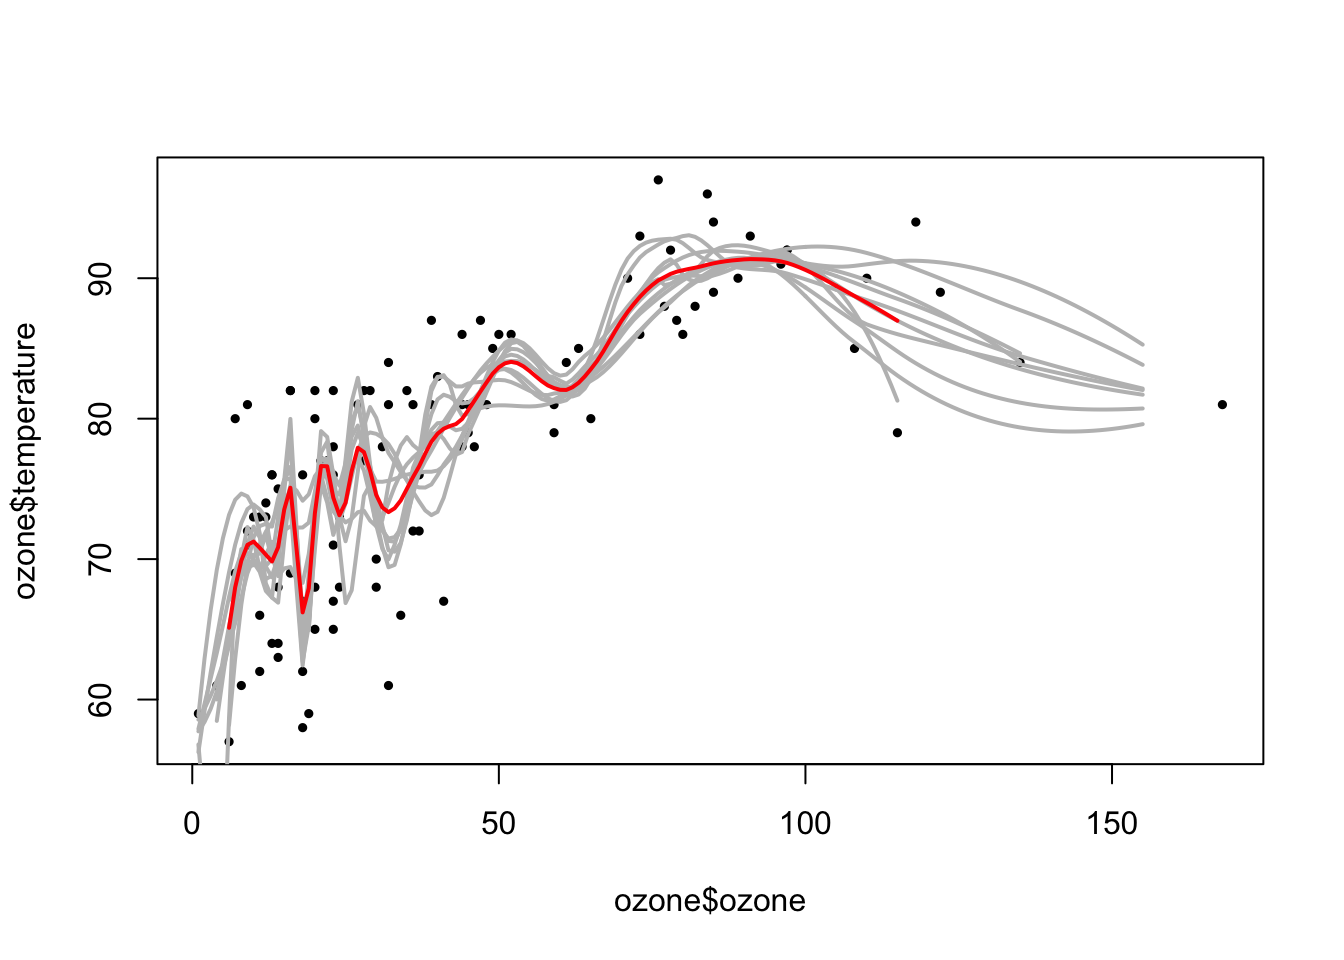
\includegraphics[width=\linewidth]{img/Ozone.png}
    \caption{De grijze lijnen zijn de voorspellingen van de verschillende algoritmen, de rode lijn is het resultaat van de \textit{ensemble}. Op de grafiek is te zien dat de uitkomst goed veralgemeniseerd is over de punten \autocite{Cen2016}.}
    \label{fig:ensemble-ozone}
\end{figure}

Met een \textit{ensemble} bedoelt men een verzameling van \textit{machine learning} algoritmes. Het gebruik van meerdere algoritmes die elkaar aanvullen leiden tot betere resultaten dan één enkel algoritme \autocite{Opitz1999}. Door de extra combinaties die nu gemaakt kunnen worden verhoogt de flexibiliteit. De simpelste manier waarop een ensemble kan werken is \textit{bagging\footnote{Ook gekend als \textit{bootstrap aggregating}.}}. Het laat elk algoritme een \textit{overfitted} voorspelling maken, de uiteindelijke uitkomst is dan het rekenkundig gemiddelde van elke voorspelling \autocite{Decorte2019}. 

Zo kan je bij \textit{random forest}, een ensemble van zoekbomen, een willekeurige factor introduceren in het trainingsproces waardoor elke zoekboom een resultaat uitkomt dat net iets van elkaar verschilt. In \textcite{Decorte2019} zien we dat combineren van al deze resultaten de performantie van het finale model verhoogt zonder dat het \textit{overfitted} is aan de trainingsdataset.

In figuur \ref{fig:ensemble-ozone} is te zien hoe \textit{bagging} tot zijn resultaat komt.

\subsection{Bayesian optimization}
\label{subsec:bayesian}

\textit{Bayesian optimization} probeert aan de hand van het probabiliteitsmodel P(score|configuratie) voorspellingen te maken over de hyperparameters \autocite{Bergstra2013}. De resultaten worden bekomen door aanpassingen te doen aan de vorige waarden van score en configuratie. In \textcite{Bergstra2013} staat dat de efficiëntie komt van het enkel overlopen van veelbelovende kandidaten uit het origineel systeem.

Desondanks er een extra abstractie laag toegevoegd wordt, is het toch bruikbaar als men honderden hyperparameters moet evalueren \autocite{Bergstra2013}.

\section{AutoML platformen}
\label{sec:automl-platformen}

\begin{figure}
    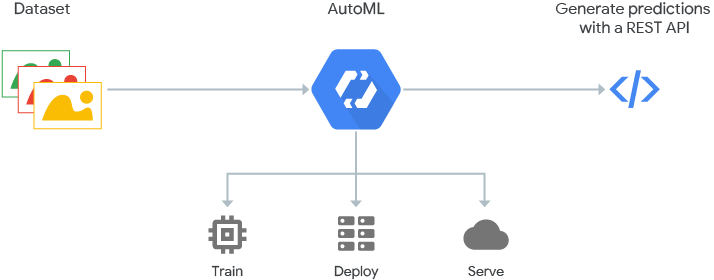
\includegraphics[width=\linewidth]{img/google-cloud-automl.png}
    \caption{Stappenplan voor een geautomatiseerd model in de cloud \autocite{Google2019}}
    \label{fig:google-cloud-automl}
\end{figure}

Het idee van geautomatiseerde toepassingen is niet nieuw, de evolutie van rekenkracht maakt het gewoon mogelijk. Er verschijnen allemaal nieuwe oplossing die runnen in de cloud of lokaal, al dan niet met grafische interfaces enzovoort. Op dit vlak is Google de koploper die het op een gebruiksvriendelijke manier aan de man brengt, maar programmeurs zijn vaak meer dan capabel om meer dan enkel een drag-en-drop systeem te gebruiken. Er zijn dan ook heel wat manieren die meer input vragen maar één bepaald aspect raken bij de gebruiker (open source, start-up, niet gecontroleerd door een groot bedrijf ...). Met deze platformen probeert de industrie de kloof tussen machine learning en een doorsnee programmeur te dichten \autocite{Gutierrez2019}.

Een open source alternatief lijkt een goede oplossing, de interfaces zijn minder gebruiksvriendelijk dan een betalend product en er komt meer programmeerwerk aan te pas. Het resultaat is vaak commercieel bruikbaar zolang de restricties van de licentie gerespecteerd worden \autocite{Balter2015}. AutoKeras is een voorbeeld onder de MIT licentie, die geen commerciële restricties oplegt. Samen met AutoKeras zijn tpot en Auto Sklearn de best ondersteunde libraries.

In deze sectie worden enkele mogelijkheden besproken.

\subsection{Google Cloud AutoML}
\label{subsec:google-automl}

Google Cloud AutoML zorgt voor een familiaire interface die een gebruiker snel op weg helpt. Naast Google hebben bedrijven zoals Microsoft en Amazon een platform gebouwd op hun respectievelijke cloud infrastructuur. De AutoML service kan voordelig zijn als het bedrijf al gebruik maakt van andere producten / diensten van de leverancier, extra kosten kunnen snel de lucht in gaan zonder toegang tot andere functies (bv. van Google Cloud) als dit niet het geval is. 

Zoals veel Google producten, heeft Cloud AutoML een familiaire interface die een gebruiker snel op weg helpt. Het proces is bijna even simpel als hun voorstelling in figuur \ref{fig:google-cloud-automl}, enkel het structureren van de dataset is niet opgenomen in de flow. De AutoML service heeft een goede kans om door te groeien in het bestaande platform van Google Cloud. De simultane werking tussen meerdere Cloud producten kan interessant zijn mocht het bedrijf gepartnered zijn met Google.

\subsubsection{Client library}
\label{subsubsec:client-library}

De beschikbare API's in de cloud worden aangesproken door HTTP requests te sturen naar de server. Een andere manier is via \textit{Client libraries\footnote{Enkel beschikbaar voor: C\#, Go, Java, Node, PHP, Python en Ruby \autocite{GoogleCLV2020}.}} die geïntegreerd worden in de code \autocite{GoogleCL2020}. De interfaces bevatten voorbeeldcode die (na setup van application keys) direct bruikbaar is om datasets en modellen te managen, modellen evalueren en (batch) voorspellingen te maken \autocite{GoogleCLV2020}. Voorspellingen van HTTP requests worden terug gestuurd als JSON, \textit{Client libraries} geven objecten in de gekozen programmeertaal met alle informatie terug.

\subsection{Microsoft Azure ML Studio}
\label{subsec:ml-studio}

Zoals bij Google Cloud AutoML zijn er ook twee manieren om aan de slag te gaan. De interface op Azure of met de Azure SDK. De \textit{client library} is enkel beschikbaar voor Python maar de werking is gelijkaardig aan sectie \ref{subsubsec:client-library} \autocite{Microsoft2020}.

\textcite{fusi2017} is de grondslag voor Azure ML Studio, het achterliggende systeem gebruikt \textit{bayesian optimization} en leunt aan bij technieken die besproken zijn in \textcite{Feurer2015}. Het bekomt een resultaat door \textit{collaborative filtering} te verwerken in \textit{hyperparameter tuning}. Hierbij wordt een voorspelling gemaakt op basis van informatie die verkregen is van een vorig getraind model die gelijkaardige keuzes vertoont. De verzamelde en geregulariseerde gegevens worden in een matrix gegoten\footnote{Deze techniek word \textit{matrix factorization} genoemd.} en kan zo gebruikt worden door het model.

\subsection{AutoKeras}
\label{subsec:autokeras}

Een AutoML systeem gebaseerd op Keras. De bedoeling van deze library is om machine learning toegankelijk te maken voor iedereen \autocite{jin2019}. AutoKeras is op dit moment nog in pre-release en kan nog sterk veranderen in de toekomst. Het gebruik is redelijk vanzelfsprekend en een volledige beschrijving van tekst en afbeeldingsanalyse zijn beschikbaar op de website. Van alle opgelijste mogelijkheden, vraagt deze library het meeste werk naast het voorzien van de data. Zo moet het model lokaal getraind worden en niet in de cloud, en moet de gebruiker een basis kennis Python hebben (om met de classifier van start te gaan). Een lokaal getraind model brengt ook wat voordelen met zich mee. Zo is er de mogelijkheid om het te exporteren naar een werkend Keras model dat nog verder aangepast kan worden. 

Voor de Image Classifier is het voorbeeld uitgewerkt met de MNIST Hand-Written Digits, zowat de standaard dataset voor afbeeldingsherkenning. Het bevat 70000 afbeeldingen van handgeschreven letters die voorzichtig opgeschoond zijn om te gebruiken als test. Ze worden vaak gebruikt bij het schrijven van de algoritmes om verbeteringen te verifiëren. Het gevolg hiervan is dat de behaalde nauwkeurigheid niet per se representatief is op realistische voorbeelden waar afbeeldingen verschillende resoluties, kleur-schalen en aspect-ratios kunnen hebben.

Achterliggend gebruikt het \textit{Neural Architecture Search} en het is aangewezen om het model te trainen op een machine met een externe grafische kaart die ondersteund wordt door de NVIDIA CUDA Toolkit.

\subsection{Auto-sklearn en TPOT}
\label{subsec:autosk}

Auto-sklearn is een open-source library die gebruik maakt van Bayesian optimization \autocite{Feurer2015}. Het optimalisatieproces gebruikt de secties die eerder besproken zijn in \ref{sec:hyperparameter-tuning} en bestaat uit volgende stappen \autocite{Feurer2016}: 

\begin{itemize}
    \item Probabiliteitsmodel bouwen die de relatie tussen hyperparameters en de performantie meet.
    \item Interessante hyperparameters selecteren door een evenwicht te zoeken tussen exploratie\footnote{Zoeken op plaatsen van de zoekruimte waar het model onzeker is.} en exploitatie\footnote{Focussen op delen van de zoekruimte die leiden tot performantie.}.
    \item Algoritme uitvoeren met de gekozen hyperparameters.
\end{itemize}

Het gegeneraliseerde proces kan gebruikt worden om algoritmes, \textit{pre-processing} methodes en hyperparameters te selecteren.

\subsubsection{Tree-based Pipeline Optimization Tool}

\textcite{Olson2016} stelt een \textit{data science} assistent voor. TPOT is een \textit{machine learning pipeline} optimalisatie tool en is niet bedoelt om het proces van begin tot eind over te nemen. Het is een technologie die meer dan een basiskennis \textit{machine learning} vergt, maar toch het vermelden waard is door het resultaat dat de gebruiker krijgt. Normaal gezien verwacht men een geëxporteerd model, bij TPOT wordt de volledige pipeline opgezet en geconverteerd naar een Python file dat nog verder geconfigureerd kan worden. Het maakt in feite een voorstel in de plaats van een definitieve keuze over de structuur van het model. 

TPOT wordt samen vermeld met Auto-sklearn omdat beide gebouwd zijn op sklearn \autocite{Olson2016}.

\section{Deployment}
\label{sec:deployment}

Voor een development team is het niet voldoende om enkel en alleen een model te trainen. Om het te kunnen gebruiken moet het ergens online staan zodat de applicatie waarin het verwerkt zit kan communiceren met het model. Bij de grote platformen zal het uitgerold worden op hun cloud services. Dat maakt nu eenmaal deel uit van hun kostenmodel. De gebruiker hangt dus in enigste zin vast aan zijn provider. 
In open source libraries is daar geen rekening mee gehouden. Een simpele oplossing is om zelf een REST API te schrijven. Er is geen beste manier omdat elke implementatie afhankelijk is van het export type van de library die je gebruikt. Om toch een representatief voorbeeld te geven wordt het deployment proces van een Keras model (export type van AutoKeras) besproken. 

Een goede strategie is om je API te bouwen in de taal waarin de library geschreven is. Zo kan je de bestaande interfaces van het geëxporteerde model direct aanspreken. In dit geval is het Python + Flask framework. Om het op een productie niveau te krijgen is het een goed idee om ook Redis\footnote{Redis is een gedistribueerde key-value store die volledige objecten in zijn geheugen kan opslaan en in deze situatie gebruikt wordt om wachtrijen te optimaliseren \autocite{Adrian2018}.} te implementeren. Dan rest enkel nog de hosting, waardoor je soms toch uitkomt bij de grote platformen zoals Amazon AWS, Google Cloud Hosting enzovoort.

In \textcite{Adrian2018} is de volledige code te vinden om stap voor stap uit te voeren wat hierboven beschreven is.
